\documentclass[tikz,border=8pt]{standalone}
\usepackage[T1]{fontenc}
\usepackage{lmodern}
\usepackage{tikz}
\usetikzlibrary{arrows.meta,positioning,calc}

\begin{document}
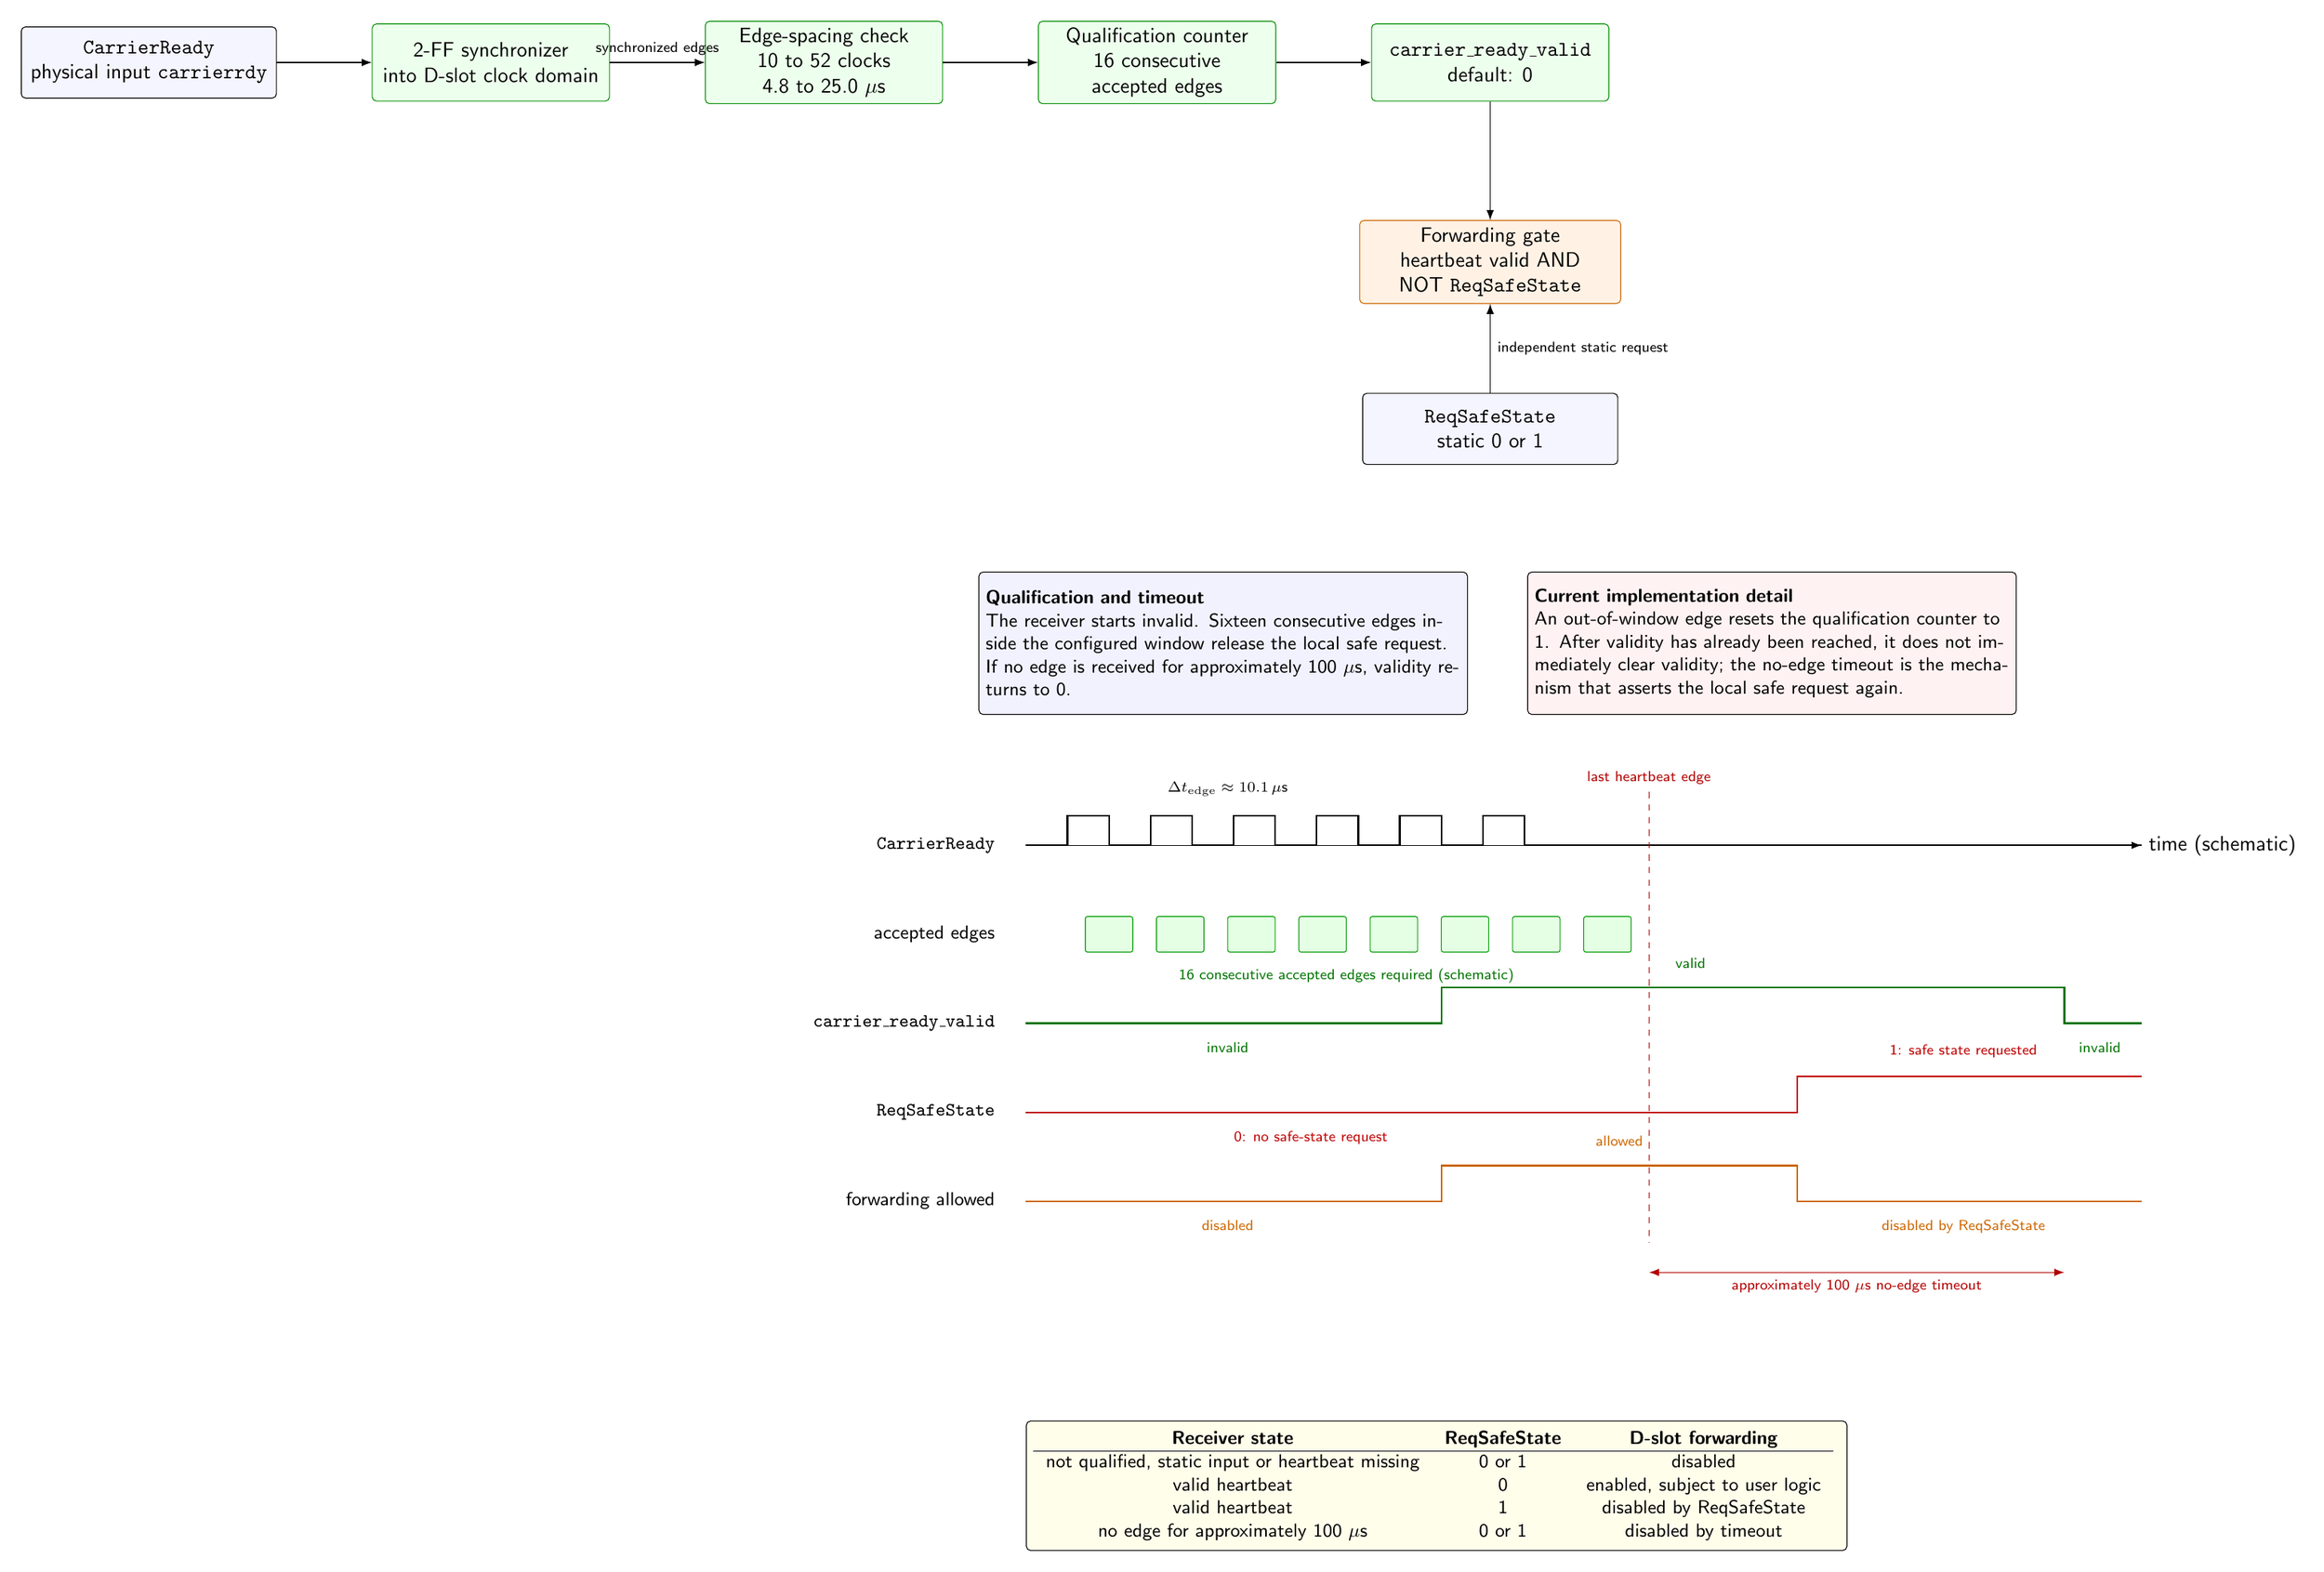
\begin{tikzpicture}[
  font=\sffamily,
  >=Latex,
  dblock/.style={draw=green!55!black, rounded corners=2pt, align=center,
                 minimum height=13mm, minimum width=40mm, fill=green!7},
  gate/.style={draw=orange!80!black, rounded corners=2pt, align=center,
               minimum height=13mm, minimum width=44mm, fill=orange!10},
  signal/.style={draw, rounded corners=2pt, align=center, minimum height=12mm,
                 minimum width=43mm, fill=blue!4},
  info/.style={draw, rounded corners=2pt, align=left, font=\sffamily\small,
               text width=80mm, minimum height=24mm},
  note/.style={font=\sffamily\small, align=center},
  tiny/.style={font=\sffamily\scriptsize, align=center},
  sig/.style={thick},
  accepted/.style={draw=green!60!black, fill=green!10, rounded corners=1pt}
]

% Receiver data path
\node[signal] (input) {\texttt{CarrierReady}\\physical input \texttt{carrierrdy}};
\node[dblock, right=16mm of input] (sync)
  {2-FF synchronizer\\into D-slot clock domain};
\node[dblock, right=16mm of sync] (window)
  {Edge-spacing check\\10 to 52 clocks\\4.8 to 25.0 $\mu$s};
\node[dblock, right=16mm of window] (counter)
  {Qualification counter\\16 consecutive\\accepted edges};
\node[dblock, right=16mm of counter] (valid)
  {\texttt{carrier\_ready\_valid}\\default: 0};

\draw[->] (input) -- (sync);
\draw[->] (sync) -- node[above,tiny] {synchronized edges} (window);
\draw[->] (window) -- (counter);
\draw[->] (counter) -- (valid);

% Separate static request and final forwarding gate
\node[gate, below=20mm of valid] (forward)
  {Forwarding gate\\heartbeat valid AND\\NOT \texttt{ReqSafeState}};
\node[signal, below=15mm of forward] (reqsafe)
  {\texttt{ReqSafeState}\\static 0 or 1};
\draw[->] (valid) -- (forward);
\draw[->] (reqsafe) -- node[right,tiny] {independent static request} (forward);

% Receiver behavior and current implementation boundary
\node[info, fill=blue!5, below=18mm of reqsafe, xshift=-45mm] (rule) {
  \textbf{Qualification and timeout}\\
  The receiver starts invalid. Sixteen consecutive edges inside the configured
  window release the local safe request. If no edge is received for approximately
  100 $\mu$s, validity returns to 0.
};
\node[info, fill=red!5, right=10mm of rule] (boundary) {
  \textbf{Current implementation detail}\\
  An out-of-window edge resets the qualification counter to 1.
  After validity has already been reached, it does not immediately clear validity;
  the no-edge timeout is the mechanism that asserts the local safe request again.
};

% Schematic timing diagram
\coordinate (t0) at ($(rule.south west)+(8mm,-22mm)$);
\draw[->] (t0) -- ++(188mm,0) node[right] {time (schematic)};
\node[note, anchor=east] at ($(t0)+(-4mm,0mm)$) {\texttt{CarrierReady}};
\node[note, anchor=east] at ($(t0)+(-4mm,-15mm)$) {accepted edges};
\node[note, anchor=east] at ($(t0)+(-4mm,-30mm)$)
  {\texttt{carrier\_ready\_valid}};
\node[note, anchor=east] at ($(t0)+(-4mm,-45mm)$)
  {\texttt{ReqSafeState}};
\node[note, anchor=east] at ($(t0)+(-4mm,-60mm)$) {forwarding allowed};

% Valid heartbeat followed by loss of edges.
\draw[sig] ($(t0)+(0,0)$)
  -- ++(7mm,0) -- ++(0,5mm) -- ++(7mm,0) -- ++(0,-5mm)
  -- ++(7mm,0) -- ++(0,5mm) -- ++(7mm,0) -- ++(0,-5mm)
  -- ++(7mm,0) -- ++(0,5mm) -- ++(7mm,0) -- ++(0,-5mm)
  -- ++(7mm,0) -- ++(0,5mm) -- ++(7mm,0) -- ++(0,-5mm)
  -- ++(7mm,0) -- ++(0,5mm) -- ++(7mm,0) -- ++(0,-5mm)
  -- ++(7mm,0) -- ++(0,5mm) -- ++(7mm,0) -- ++(0,-5mm)
  -- ++(21mm,0) -- ++(83mm,0);
\draw[dashed, red!70!black] ($(t0)+(105mm,9mm)$) -- ($(t0)+(105mm,-67mm)$);
\node[tiny, red!70!black, anchor=south] at ($(t0)+(105mm,9mm)$)
  {last heartbeat edge};
\node[tiny, anchor=south] at ($(t0)+(34mm,7mm)$)
  {$\Delta t_{\mathrm{edge}}\approx10.1\,\mu$s};

\foreach \x in {10,22,34,46,58,70,82,94} {
  \draw[accepted] ($(t0)+(\x mm,-18mm)$) rectangle ++(8mm,6mm);
}
\node[tiny, green!45!black] at ($(t0)+(54mm,-22mm)$)
  {16 consecutive accepted edges required (schematic)};

% Active-high validity.
\draw[sig, green!45!black] ($(t0)+(0,-30mm)$) -- ++(70mm,0)
  -- ++(0,6mm) -- ++(105mm,0)
  -- ++(0,-6mm) -- ++(13mm,0);
\node[tiny, green!45!black, anchor=north] at ($(t0)+(34mm,-32mm)$) {invalid};
\node[tiny, green!45!black, anchor=south] at ($(t0)+(112mm,-22mm)$) {valid};
\node[tiny, green!45!black, anchor=north] at ($(t0)+(181mm,-32mm)$) {invalid};

% ReqSafeState independently disables forwarding before heartbeat timeout.
\draw[sig, red!75!black] ($(t0)+(0,-45mm)$) -- ++(130mm,0)
  -- ++(0,6mm) -- ++(58mm,0);
\node[tiny, red!75!black, anchor=north] at ($(t0)+(48mm,-47mm)$)
  {0: no safe-state request};
\node[tiny, red!75!black, anchor=south] at ($(t0)+(158mm,-37mm)$)
  {1: safe state requested};

\draw[sig, orange!80!black] ($(t0)+(0,-60mm)$) -- ++(70mm,0)
  -- ++(0,6mm) -- ++(60mm,0)
  -- ++(0,-6mm) -- ++(58mm,0);
\node[tiny, orange!80!black, anchor=north] at ($(t0)+(34mm,-62mm)$) {disabled};
\node[tiny, orange!80!black, anchor=south] at ($(t0)+(100mm,-52mm)$) {allowed};
\node[tiny, orange!80!black, anchor=north] at ($(t0)+(158mm,-62mm)$)
  {disabled by ReqSafeState};

\draw[<->, red!70!black] ($(t0)+(105mm,-72mm)$)
  -- node[below,tiny] {approximately 100 $\mu$s no-edge timeout}
     ($(t0)+(175mm,-72mm)$);

% Truth table
\node[draw, rounded corners=2pt, fill=yellow!8, align=center,
      font=\sffamily\small, below=25mm of t0, yshift=-72mm, anchor=north west] {
\begin{tabular}{c c c}
\textbf{Receiver state} & \textbf{ReqSafeState} & \textbf{D-slot forwarding}\\
\hline
not qualified, static input or heartbeat missing & 0 or 1 & disabled\\
valid heartbeat & 0 & enabled, subject to user logic\\
valid heartbeat & 1 & disabled by ReqSafeState\\
no edge for approximately 100 $\mu$s & 0 or 1 & disabled by timeout
\end{tabular}
};

\end{tikzpicture}
\end{document}
